\documentclass[aps, pre, onecolumn, nofootinbib, notitlepage, groupedaddress, amsfonts, amssymb, amsmath, longbibliography]{revtex4-1}
\usepackage{tabularx}
\usepackage{graphicx}
\usepackage{hyperref}
\usepackage{xcolor}
\hypersetup{
    colorlinks,
    linkcolor={red!50!black},
    citecolor={blue!50!black},
    urlcolor={blue!80!black}
}
\usepackage{bm}
\usepackage{natbib}
\usepackage{longtable}
\LTcapwidth=0.87\textwidth

\newcommand{\Div}[1]{\ensuremath{\nabla\cdot\left( #1\right)}}
\newcommand{\DivU}{\ensuremath{\nabla\cdot\bm{u}}}
\newcommand{\angles}[1]{\ensuremath{\left\langle #1 \right\rangle}}
\newcommand{\KS}[1]{\ensuremath{D_{\text{KS}}(#1)}}
\newcommand{\KSstat}[1]{\ensuremath{\overline{D_\text{KS}(#1)}}}
\newcommand{\grad}{\ensuremath{\nabla}}
\newcommand{\RB}{Rayleigh-B\'{e}nard }
\newcommand{\Reff}{\ensuremath{\text{Re}_{\text{ff}}}}
\newcommand{\Peff}{\ensuremath{\text{Pe}_{\text{ff}}}}


\newcommand\mnras{{MNRAS}}%

\begin{document}
\author{Evan H. Anders}
\affiliation{Dept. Astrophysical \& Planetary Sciences, University of Colorado -- Boulder, Boulder, CO 80309, USA}
\affiliation{Laboratory for Atmospheric and Space Physics, Boulder, CO 80303, USA}
\author{Geoffrey M. Vasil}
\affiliation{University of Sydney School of Mathematics and Statistics, Sydney, NSW 2006, Australia}
\author{Benjamin P. Brown}
\affiliation{Dept. Astrophysical \& Planetary Sciences, University of Colorado -- Boulder, Boulder, CO 80309, USA}
\affiliation{Laboratory for Atmospheric and Space Physics, Boulder, CO 80303, USA}
\author{Lydia Korre}
\affiliation{Laboratory for Atmospheric and Space Physics, Boulder, CO 80303, USA}
\author{Jeffrey S. Oishi}
\affiliation{Department of Physics and Astronomy, Bates College, Lewiston, ME 04240, USA}

\title{Mixed thermal boundary conditions impose an unnecessary thermal rundown on convection simulations}

\begin{abstract}
Astrophysical studies of convection often impose different thermal boundary conditions at the top and the bottom of the domain in an effort to more accurately reflect the natural system being modeled.
In this work, we study \RB convection (RBC) to show that the use of these mixed thermal boundary conditions imposes a long thermal rundown on convective systems which is not experienced by the more classical system where the temperature is fixed at the top and bottom of the domain.
We demonstrate that the mean behavior of an evolved simulation with mixed thermal boundaries corresponds to an equivalent simulation with fixed temperature boundaries at the top and bottom.
We show that the fast evolution of fixed-temperature simulations can be taken advantage of to rapidly relax simulations with mixed boundaries.
In the measurements presented here, we find that the asymmetries created by mixed boundaries do not importantly affect spatially averaged dynamics, but we do find that more extreme values of temperature can occur near a fixed flux boundary than a fixed temperature boundary.
We also demonstrate that these findings carry over to more complicated problems through a brief examination of rotating convection.
These results suggest that thermal relaxation occurs in two stages: (1) changes to the experimental energy reservoir and (2) changes to the stratification of the experiment.
Through the proper choice of boundary conditions or initial conditions, the first of these stages can be bypassed, and the second stage seems to be irrelevant for RBC.
\end{abstract}
\maketitle

%%%%%%%%%%%%
%%%%%%%%%%%
% INTRO
%%%%%%%%%%%
%%%%%%%%%%%%

\section{Introduction}
\label{sec:introduction}
Convection is a crucial heat transport mechanism in the atmospheres and interiors of stars and planets.
Numerical simulations are the basis for most modern studies into the nature of astrophysical convection.
Some modern studies examine convection in the highly simplified Boussinesq approximation \cite{spiegel&veronis1960}.
Others study more complex ``dynamo simulations'', incorporating complicating effects such as magnetism and atmospheric density stratification \cite{charbonneau2014, toomre2019}.
Regardless of the degree of apparent realism included in these models, convective processes in these numerical simulations are fundamentally driven by some combination of imposed boundary conditions and internal heating profiles which in turn determine key properties of the evolved dynamics \cite{goluskin2015}.
In astrophysical studies, a common choice of thermal boundary conditions \cite{glatzmaier&gilman1982, hurlburt&all1986, cattaneo&all1990, featherstone&hindman2016a, korre&all2019, wood&brummell2018, kapyla&all2019} is to fix the flux at the bottom boundary and to fix the value of a thermodynamic quantity (e.g., temperature) at the top boundary.
In this work, we will examine the consequences of these ``mixed'' boundaries in the simplest possible model: \RB convection under the Boussinesq approximation.
In this model, the only thermodynamic quantity of interest is the temperature, and we will hereafter refer to this choice of boundary conditions (fixed flux at the bottom, fixed temperature at the top) as ``mixedFT'' boundaries.

Despite mixedFT boundary conditions being a common choice of numericists, we are unaware of any work which compares the dynamics produced by mixed thermal boundaries to the most traditional choice of boundary conditions in the \RB literature: fixed temperature at the top and bottom (hereafter ``fixedT'' boundaries).
Due to the fact that mixedFT boundaries fix the flux through the convective system, this set of boundaries is expected to behave in a fundamentally similar way to a system in which the flux is fixed at both boundaries (hereafter ``fixedF'' boundaries), whose behavior is well-known \cite{otero&all2002, goluskin2015}.
While there is some work \cite{johnston&doering2009} comparing fixedF and fixedT boundaries, past work primarily focused on the scaling of heat transport laws (quantified by a Nusselt number, Nu) as the convective driving is increased (quantified by the Rayleigh number, Ra) [more refs].
The equivalence of fixedF and fixedT scaling laws suggests that mixedFT scaling should also be identical.
However, the choice of mixedFT boundaries introduces complexities into the convective system which neither fixedF or fixedT boundaries are exposed to.
First, the evolved mean temperature of a simulation with mixedFT boundaries differs from the initial mean temperature, and therefore the thermal reservoir of the convective system must evolve over time.
Second, mixedFT boundary conditions are fundamentally asymmetric, and the degree to which these boundary conditions break the symmetry of the system is unclear.

In this paper, we investigate the time evolution and nature of asymmetries in \RB covection when mixedFT boundary conditions are imposed.
We find that the thermal evolution and relaxation of mixedFT systems is very long compared to fixedT systems, where it is nearly instantaneous.
We also find that this rapid thermal evolution can be bypassed by combining the results of fixedT and mixedFT simulations.
We furthermore find that the choice of mixedFT boundaries imposes some asymmetries on the convective flows, but that these asymmetries do not seem to appreciably change the mean convective state when compared to fixedT boundaries, even when the Rayleigh number is large.
We present these findings as follows.
In section \ref{sec:simulations}, we describe our experimental setup and numerical methods.
In section \ref{sec:results}, we first describe our findings with respect to the time evolution of mixedFT systems, and then describe the asymmetries in these systems.
In section \ref{sec:rotating_results}, we briefly show that these findings carry over to a more complex system: rotating \RB convection.
Finally, in section \ref{sec:discussion}, we briefly describe the implications of this work for the field of astrophysical convection.

%%%%%%%%%%%%
%%%%%%%%%%%
% EXPERIMENT
%%%%%%%%%%%
%%%%%%%%%%%%

\section{Simulation Details}
\label{sec:simulations}
We study incompressible \RB convection under a freefall nondimensionalization as we have done previously \cite{anders&all2018}; for details of the nondimensionalization, we refer readers to that previous work.
In section \ref{sec:rotating_results} we study convection which includes the effects of vertical global rotation \cite{julien&all1996}, so we include it here for generality.
The equations of motion are
\begin{align}
\Div{\bm{u}} &= 0
	\label{eqn:incompressible}
\\
\frac{\partial \bm{u}}{\partial t} + \left(\bm{\omega} + \frac{1}{\text{Ek }\Reff}\hat{z}\right)\times\bm{u} 
&= - \grad \varpi + T_1\hat{z} - \frac{1}{\Reff}\grad\times\bm{\omega},
	\label{eqn:bouss_momentum}
\\
\frac{\partial T_1}{\partial t}  + \bm{u}\cdot\grad T_1 + w \frac{\partial T_0}{\partial z} 
&= \frac{1}{\Peff}\grad^2 T_1,
	\label{eqn:bouss_energy}
\end{align}
where $\bm{u} = (u, v, w)$ is the velocity, $T = T_0(z) + T_1(x, y, z, t)$ is the temperature (where $T_0$ is the initial profile and $T_1$ is the fluctuations around that profile), $\varpi = [defn]$ is the reduced pressure which enforces the incompressible constraint, and $\bm{\omega} = \grad \times \bm{u}$ is the vorticity.
The dimensionless control parameters are the Rayleigh, Prandtl, and Ekman numbers,
\begin{equation}
\text{Ra} = \frac{g \alpha L_z^3 \Delta}{\nu\kappa} = \frac{(L_z\,v_{\text{ff}})^2}{\nu\kappa}, \qquad \text{Pr} = \frac{\nu}{\kappa}, \qquad \text{Ek} = \sqrt{\frac{\nu}{2\Omega L_z^2}},
\end{equation}
where $g$ is the gravity, $\alpha$ is the coefficient of thermal expansion, $L_z$ is the domain depth, $\nu$ and $\kappa$ are respectively the viscous and thermal diffusivity, and $\Omega$ is the global rotation frequency \cite{anders&all2018}.
These parameters set the freefall Reynolds and Peclet numbers, $\Reff = \sqrt{\text{Ra}/\text{Pr}}$ and $\Peff = \text{Pr }\Reff$, and throughout this work we hold Pr = 1 so that $\Reff = \Peff$.
In our cases where rotation is not included, we set Ek$\,= \infty$.
The extent of our numerical domain is $z = [-0.5, 0.5]$ vertically and $x, y = [-\Gamma/2, \Gamma/2]$, where $\Gamma$ is the aspect ratio.
The initial temperature profile, $T_0(z) = 0.5 - z$, is unstable and linearly decreases from a value of 1 to 0 across the domain. 
$\Delta$ is the dimensionless temperature jump across the domain; depending on our choice of boundary condition, $\Delta$ defines either a temperature or flux Rayleigh number,
\begin{equation}
\text{Ra}_{\Delta T} = \frac{g \alpha L_z^3 \Delta T_0}{\nu\kappa}, \qquad 
\text{Ra}_{\partial_z T} = \frac{g \alpha L_z^4 \partial_z T_0}{\nu\kappa}.
\end{equation}


Throughout the bulk of this work, we study two-dimensional (2D) convection where $\partial_y = v = 0$.
For comparison with the literature, we specify $\Gamma = 2$ and these simulations employ no-slip, impenetrable boundaries,
\begin{equation}
u = w = 0 \, \, \text{at}\,\,z = -0.5, 0.5.
\label{eqn:vel_bcs}
\end{equation}
The rotating cases in section \ref{sec:rotating_results} are three-dimensional (3D) tall, skinny boxes with $\Gamma = 10\lambda_c(\text{Ek})$, where $\lambda_c(\text{Ek})$ is the wavelength of convective onset, as has been done by previous authors \cite{stellmach&all2014}. 
These rotating simulations employ stress-free, impenetrable boundaries,
\begin{equation}
\partial_z u = \partial_z v = w = 0 \, \, \text{at}\,\,z = -0.5, 0.5.
\label{eqn:vel_bcs}
\end{equation}
We study both mixedFT and fixedT thermal boundary conditions,
\begin{equation}
(\text{mixedFT}): T_1 = 0 \text{ at $z$ = 0.5} \,\&\, \partial_z T_1 = 0 \text{ at $z$ = -0.5};\qquad\qquad
(\text{fixedT}): T_1 = 0 \text{ at $z$ = -0.5, 0.5}.
\end{equation}
In the case of mixedFT boundaries, the temperature is nondimensionalized on the initial temperature gradient, $\Delta = L_z \partial_z T_0$, and the input Rayleigh number is a flux Rayleigh number, Ra$_{\partial_z T}$.
In the case of fixedT boundaries, the temperature is nondimensionalized on the initial temperature jump across the domain: $\Delta = \Delta T_0 =  T_0(z=0.5)-T_0(z=-0.5)$, and the input Rayleigh number is a temperature Rayleigh number, Ra$_{\Delta T}$.

We utilize the Dedalus\footnote{\url{http://dedalus-project.org/}} pseudospectral framework \cite{burns&all2016, burns&all2019} to evolve Eqs.~(\ref{eqn:incompressible}-\ref{eqn:bouss_energy}) forward in time.
Our 2D simulations use an implicit-explicit (IMEX), third-order, four-stage Runge-Kutta timestepping scheme RK443; our 3D simulations use the second-order, two-stage Runge-Kutta scheme RK222 \cite{ascher&all1997}. 
The code used to run simulations and the code and data used to create the figures in this work are available publicly online in a repository of supplemental materials \cite{anders&all2020a_supp}.
Variables are time-evolved on a dealiased Chebyshev (vertical) and Fourier (horizontal, periodic) domain in which the physical grid dimensions are 3/2 the size of the coefficient grid.  
We fill $T_1$ with random white noise whose magnitude is $10^{-6}/\Peff$, and which is vertically tapered to zero at the boundaries.
We filter this noise spectrum in coefficient space, such that only the lower 25\% of the coefficients have power; this low-pass filter is used to avoid populating the highest wavenumbers with noise in order to improve the stability of our spectral timestepping methods.


%%%%%%%%%%%%%%%%%%%%%%%%%%%%%%%%%%%%
%%%%%%%%%%%%%%%%%%%%%%%%%%%%%%%%%%
% Ra & Nu arguments
%%%%%%%%%%%%%%%%%%%%%%%%%%%%%%%%%%
%%%%%%%%%%%%%%%%%%%%%%%%%%%%%%%%%%%%
\subsection{Nondimensional Output Quantities}
\label{sec:ra_nu_relations}
Throughout this work we will measure and report the evolved value of the Nusselt number.
We define and measure the Nusselt number instantaneously as
\begin{equation}
\text{Nu} \equiv \angles{\frac{w T - \Peff^{-1} \partial_z T}{-\Peff^{-1} \angles{\partial_z T}}}
= 1 + \Peff\frac{\angles{w T}}{-\Delta T},
\end{equation}
where $\angles{}$ represent a volume average ($\angles{A} \equiv \iint A\,dx\,dz / \Gamma$ in 2D and $\angles{A} \equiv \iiint A\,dx\,dy\,dz / \Gamma^2$ in 3D for some quantity $A$), and $\Delta T = \angles{\partial_z T}$ is the temperature difference between the top and bottom plate.
In the evolved, statistically stationary state, when fixedT boundaries are employed, $\text{Nu} = 1 + \Peff\angles{wT} = \text{(Evolved Flux)}$, and when mixedFT boundaries and a flux nondimensionalization are employed, $\text{Nu} = (\Delta T)^{-1}$.
This suggests that the equilibrated state of a given convective solution is characterized by both a flux and temperature Rayleigh number whose relationship is
\begin{equation}
\text{Ra}_{\partial_z T} = \text{Ra}_{\Delta T} \text{Nu}.
\label{eqn:ra_relation}
\end{equation}
In other words, in addition to measuring the efficiency of convective heat transport, the Nusselt number is also the unit of conversion between a temperature and a flux nondimensionalization in the evolved state.

Some additional quantities of interest will be reported throughout this paper.
We will measure the evolved Peclet number of the convective flows in all sections, and in section \ref{sec:rotating_results} we will also report the value of the Rossby number.
We measure these nondimensional quantities instantaneously as
\begin{equation}
\text{Pe} = \angles{|\bm{u}|}\Peff,\qquad \text{Ro} = \angles{|\bm{\omega}|}\text{Ek }\Reff,
\end{equation}
where $|\bm{A}|$ represents the magnitude of the vector $\bm{A}$.





%%%%%%%%%%%%
%%%%%%%%%%%
% RESULTS
%%%%%%%%%%%
%%%%%%%%%%%%
\section{Results}
\label{sec:results}

\subsection{Time Evolution}
\label{sec:2d_results}

\begin{figure}
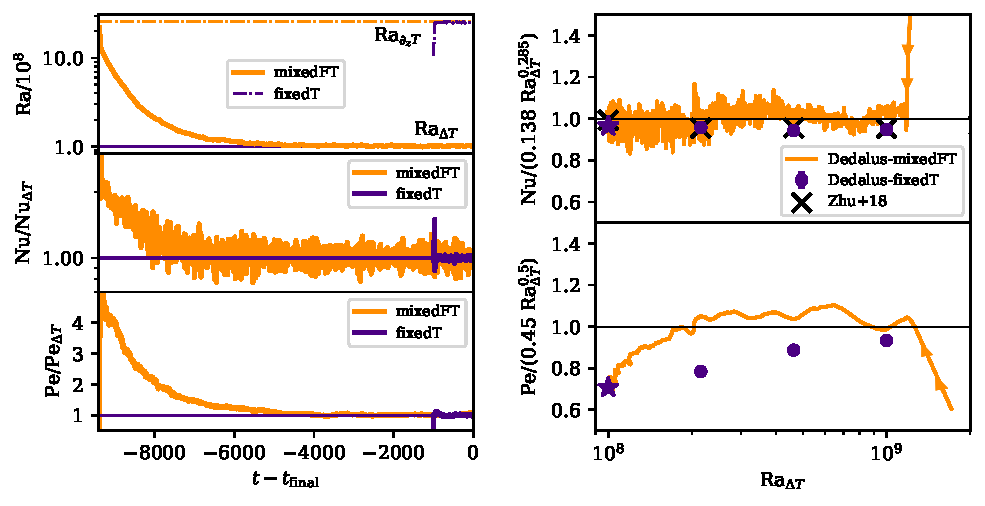
\includegraphics[width=\textwidth]{./figs/rbc_scalar_comparisons.pdf}
\caption{ 
	(left three panels) Time traces of rolling averages over 50 freefall times of a mixedFT simulation (green) and a fixedT (orange) simulation.
	(top left panel) The Rayleigh number, normalized by the input Ra$_{\partial_z T}$ = 2.61$\,\times 10^9$ value of the mixedFT simulation.
	(middle and bottom left panels) The Nusselt number and Peclet number evolution of the simulations is shown, and is normalized by the mean value measured over the last 500 freefall times of the fixedT simulation.
	(right two panels) Parameter space plots of Nusselt (upper) and Peclet (lower) vs. Ra$_{\Delta T}$.
	The green traces show the time evolution of the mixedFT case, while the orange circles and black crosses show comparison fixedT simulations.
	The orange star in each plot corresponds to the fixedT case whose time evolution is shown on the left.
\label{fig:rbc_scalar_comparisons} }
\end{figure}

In Fig.~\ref{fig:rbc_scalar_comparisons}, we describe the evolution of a mixedFT simulation which is characterized by Ra$_{\partial_z T}$ = 2.61$\,\times 10^9$.
This simulation had a coefficient resolution of (nz, nx) = (1024, 2048) and was evolved forward in time for ten days on 512 cpus.
The left panels of Fig.~\ref{fig:rbc_scalar_comparisons} compare this simulation to a fixedT case with Ra$_{\Delta T} = 10^8$, with a coefficient resolution of (nz, nx) = (512, 1024) which was time evolved for one thousand freefall time units after the initial convective transient (which took roughly one day on 256 cpus).
The mixedFT case is displayed in green, and the fixedT case is displayed in orange; the x-axis of the left panels shows simulation time, in freefall units, with the time of the simulation's end subtracted from it (such that $x = 0$ corresponds to the end of the simulation).
In the top-left panel, we compare the evolution of the Rayleigh number of these simulations: temperature Rayleigh numbers, Ra$_{\Delta T}$ are displayed as solid lines, and flux Rayleigh numbers, Ra$_{\partial_z T}$ are shown as dash-dot lines.
The value of Ra$_{\Delta T}$ takes thousands of time units to reach its final value for the mixedFT simulation, and this final value corresponds to the input value of the equivalent fixedT case.
On the other hand, the value of Ra$_{\partial_z T}$ for the fixedT case nearly instantaneously reaches its final value, which corresponds to the input value for the mixedFT simulation.
This discrepancy in evolution timescales, where fixedT simulations evolve quickly and mixedFT simulations evolve slowly, is also seen in the equilibration of the Nusselt number (middle panel) and Peclet number (bottom panel).
All time traces displayed are rolling averages over 50 freefall times, in order to reduce the variance of the plotted quantities.

In the right panels of Fig.~\ref{fig:rbc_scalar_comparisons}, we plot Nu and Pe vs Ra$_{\Delta T}$.
The green line shown in each panel is the path through parameter space that the mixed-FT simulation traces out over its time evolution.
In the upper right (Nu vs Ra) plot, we have divided all Nu values by $(0.138 \text{Ra}_{\Delta T}^{0.285})$, which was the best-fit reported by \cite{johnston&doering2009}.
In the lower right (Re vs Ra) plot, we have divided out a Ra$_{\Delta T}^{1/2}$ law, which is the anticipated scaling of the Peclet number \cite{ahlers&all2009}.
The orange circles show the mean values of Nu and Pe from select fixedT simulations through this parameter space, the details of which are presented in appendix \ref{app:table}; in all cases, we plot the sample mean, and the standard deviation of the sample mean is smaller than the plotted points.
The orange star is the simulation whose time evolution is shown on the left.
The black crosses are the reported values of Nu from the supplemental materials of \cite{zhu&all2018}, presented for comparison.
Remarkably, the mixedFT case seems to reliably perform a sweep through this parameter space.
However, despite seemingly tracing out the ``proper'' values of Nu(t) vs. Ra$_{\Delta T}$(t), we find that the mixedFT simulation achieves a larger value of the Peclet number than the comparison fixedT simulations until it converges to its final state.
These traces through parameter space help to demonstrate the importance of waiting until a mixedFT simulation has reached its equilibrated state.

\begin{figure}
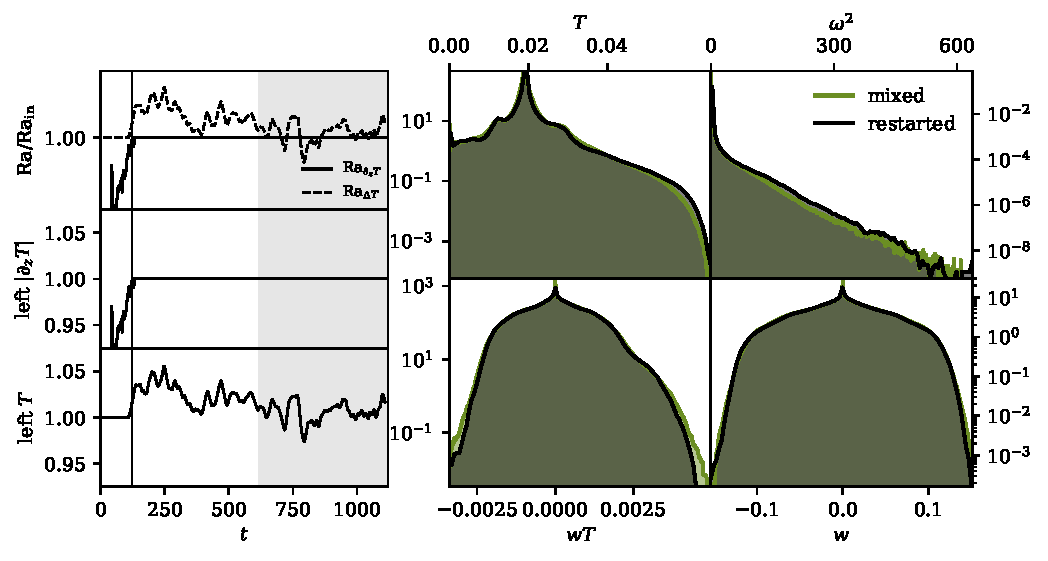
\includegraphics[width=\textwidth]{./figs/rbc_restart_description.pdf}
\caption{ 
	(left three panels) Time traces of rolling averages over 25 freefall times of a simulation which starts with fixedT boundary conditions and then is switched to mixedFT boundary conditions.
	(top left panel) The Rayleigh number's evolution over time is shown; Ra$_{\partial_z T}/(2.61\times 10^9)$ is shown as a dashed-dot line, while Ra$_{\Delta T}/10^8$ is shown as a solid line.
	The mean value of the simulation's temperature gradient (middle panel) and temperature (bottom panel) are displayed, showing the change in the enforced boundary condition.
	In the middle panel, during the fixedT portion of the simulation, we plot $\angles{Nu}\partial_z T$, while in the bottom panel, during the mixedFT portion, we plot $T / \angles{Nu}$ due to the change in temperature nondimensionalization for the different boundary conditions.
	(right four panels) Probability distribution functions of dynamics at all spatial points in the domain sampled once each freefall time for a total of 500 freefall times are shown.
	We display the temperature field (upper left), enstrophy (upper right), nonlinear convective enthalpy flux (bottom left), and vertical velocity (bottom right).
	In each plot, we show the PDF of the dynamics at the end of the mixedFT simulation that experienced a long rundown (green lines in Fig.~\ref{fig:rbc_scalar_comparisons}), as well as dynamics from the grey shaded region displayed in the left three panels here.
\label{fig:rbc_restart_description} }
\end{figure}

The equivalence of the evolved values of Ra, Nu, and Pe in Fig.~\ref{fig:rbc_scalar_comparisons} suggests that, in a volume-averaged sense, there is a comparable fixedT experiment for each mixedFT experiment.
It seems plausible that one should be able to take advantage of the fast evolution on display in fixedT simulations to achieve rapidly equilibrated mixedFT simulations.
The rundown in mixedFT simulations is very costly: not only do the turbulent dynamics at the large initial Rayleigh number need to be resolved (requiring more spectral modes to run the simulation), but thousands of freefall times must pass before convergence.
For a sense of scale, the first thousand freefall time units of the mixedFT case displayed in Fig.~\ref{fig:rbc_scalar_comparisons} took $1.43\times10^6$ iterations, or roughly $3.3 \times 10^4$ cpu-hours.
For comparison, the same time evolution (essentially the whole simulation) for fixedT boundary conditions took  $8.4\times10^5$ iterations, or roughly $5.4\times 10^3$ cpu-hours.
After these thousand freefall time units, the fixedT simulation has spent hundreds of freefall times in a statistically stationary state, whereas the mixedFT system continues to evolve towards its equilibrium state for an additional few thousands of time units.
This means that at these modest Rayleigh numbers (Ra$_{\Delta T} = 10^8$), the cost of equilibration of a mixedFT simulation is more than an order of magnitude larger than a fixedT simulation.

We now describe a procedure which takes advantage of the fast evolution of fixedT simulations to achieve equilibrated mixedFT simulations.
In essence, the full evolved flow fields in the fixedT simulation are properly re-nondimensionalized and fed into a mixedFT simulation as initial conditions.
More precisely, the procedure for achieving converged mixedFT dynamics using fixedT simulations takes place over these steps:
\begin{enumerate}
\item Run a fixedT simulation from convective transient to its statistically stationary state. 
Measure $\angles{\text{Nu}}$ in that state.
\item Re-nondimensionalize from $\Delta = \Delta T$ to $\Delta = L_z \partial_z T$ in the definition of the Rayleigh number.
This means changing from an input of Ra$_{\Delta T}$ to Ra$_{\partial_z T}$ as in Eqn.~\ref{eqn:ra_relation}.
In our freefall nondimensionalization, this means setting the velocities in the mixedFT simulation to $\bm{u}_{\text{mixedFT}} = \bm{u}_{\text{fixedT}} / \sqrt{\angles{\text{Nu}}}$, and setting the temperature field to $T_{\text{mixedFT}} = T_{\text{fixedT}} / \angles{\text{Nu}}$.
\item Restart the simulation with mixedFT boundaries and continue timestepping.
\end{enumerate}

In the left panels of Fig.~\ref{fig:rbc_restart_description}, we show time traces of a simulation in which we employ this procedure.
We initialize a fixedT simulation at Ra$_{\Delta T} = 10^8$, which has been reported to have $\text{Nu} \approx 26.1$ \cite{zhu&all2018}.
Roughly one hundred freefall times after the convective transient, we restart this simulation using mixedFT boundaries according to our above procedure with an input Ra$_{\partial_z T} = 2.61 \times 10^9$, and we run this simulation for a further thousand time units.
We note that this is the same Ra$_{\partial_z T}$ as the mixedFT case presented in the green lines in Fig.~\ref{fig:rbc_scalar_comparisons}.
In the upper left panel, rolling averages over 25 freefall times of Ra$_{\Delta T} / 10^8$ and Ra$_{\partial_z T} / (2.61 \times 10^9)$ are shown in the through the full simulation.
The time at which we switch from fixedT to mixedFT boundaries is noted by the vertical black line.
In the middle and bottom panels, we show the time evolution of the instantaneous temperature derivative and temperature value at the bottom plate.
In the fixedT initial state, the temperature is held constant at a value of 1 and the temperature derivative fluctuates around a value of $\angles{\text{Nu}}$.
In the mixedFT final state, the temperature derivative is held constant at a value of 1 and the temperature value fluctuates around a value of $\angles{\text{Nu}}^{-1}$.
Unlike in the mixedFT case displayed in Fig.~\ref{fig:rbc_scalar_comparisons}, there is no long thermal rundown in the mixedFT state, as the thermal profile was rapidly relaxed by the early fixedT portion of the run.

While these time traces show that this procedure bypasses the long thermal rundown on display in Fig.~\ref{fig:rbc_scalar_comparisons}, this does not prove that the dynamics in the final state are equivalent.
We now compare probability distribution functions (PDFs) of various quantities in our restarted mixedFT simulation to the mixedFT simulation that stepped through a long rundown.
For the last 500 freefall times of each simulation (e.g., the grey shaded region in Fig.~\ref{fig:rbc_restart_description}), we sample the full flow field once each freefall time.
We interpolate the (unevenly spaced) vertical chebyshev gridpoints onto an evenly spaced grid before histogramming flow values using 500 bins.
In the right four panels of Fig.~\ref{fig:rbc_restart_description}, we display PDFs of the temperature field (upper left), enstrophy (upper right), convective flux (lower left), and vertical velocity (lower right).
In Table~\ref{table:pdf_values}, we display the first four moments of each of these distributions,
\begin{equation}
\begin{split}
&\mu(A) \equiv \sum_{i} A_i\,P(A_i)\,\Delta A,\qquad\qquad\qquad\qquad\qquad\qquad\,\,
\sigma(A) \equiv \sqrt{\sum_{i}[A_i-\mu(A)]^2 P(A_i) \Delta A},\\
&\text{Skewness}(A) \equiv \frac{1}{\sigma(A)^3}\sum_i [A_i-\mu(A)]^3 P(A_i) \Delta A,\qquad
\text{Kurtosis}(A) \equiv \frac{1}{\sigma(A)^4}\sum_i [A_i-\mu(A)]^4 P(A_i) \Delta A,
\end{split}
\label{eqn:pdf_moments}
\end{equation}
where $A$ is the quantity, $P(A)$ is the PDF of quantity $A$, $\mu$ is the mean, $\sigma$ is the standard deviation, $\Delta A$ is the spacing between the PDF bins, and $i$ is the index of the bin..
Visually the PDFs of dynamics in a mixedFT and a restarted fixedT-to-mixedFT simulation are essentially identical.
In all cases except for the enstrophy, the four moments of the PDFs between the two runs are also very similar.
These simulations have no-slip boundaries, so the enstrophy is concentrated near the plume impacting sites within the boundary layers.
The small differences between the enstrophy PDFs perhaps points to slightly different plume morphologies being sampled during the 500 freefall time units in the two runs, but the similarities between the two cases in other important quantities (specfically in nonlinear transport) lead us to believe that this difference is unimportant.

\begin{table}[t!]
\caption{ 
	The first four moments, as defined in Eqn.~\ref{eqn:pdf_moments}, of each of the PDFs shown in Fig.~\ref{fig:rbc_restart_description} are displayed below.
}
\setlength{\tabcolsep}{12pt}
\label{table:pdf_values}
\begin{center}
\begin{tabularx}{\textwidth}{c c c c c c}
\hline																	
Quantity &	Case	&	$\mu$	&	$\sigma$	&	Skewness	&	Kurtosis \\
%\hline \hline \multicolumn{6}{c}{\vspace{-0.2cm}}\\
%\multicolumn{6}{c}{\vspace{0.1cm}2D Runs} \\
\hline
$T$				&	mixedFT		&		$1.9 \times 10^{-2}$	&	$4.3 \times 10^{-3}$	&	1.1		&	15 \\
				&	mixedFT,r	&		$1.9 \times 10^{-2}$	&	$4.3 \times 10^{-3}$	&	1.3		&	18 \\
\hline
$\omega^2$		&	mixedFT		&		$1.3$					&	$6.4$					&	19		&	$5.2 \times 10^2$ \\
				&	mixedFT,r	&		$3.9$					&	$7.4$					&	18		&	$4.5 \times 10^2$ \\
\hline
$wT$			&	mixedFT		&		$1.9 \times 10^{-5}$	&	$9.4 \times 10^{-4}$	&	0.16	&	$3.1$ \\
				&	mixedFT,r	&		$1.9 \times 10^{-5}$	&	$9.3 \times 10^{-4}$	&	0.16	&	$3.1$ \\
\hline
$w$				&	mixedFT		&		$7.9 \times 10^{-7}$	&	$4.9 \times 10^{-2}$	&	0.016	&	$2.7$ \\
				&	mixedFT,r	&		$-5.2 \times 10^{-6}$	&	$4.8 \times 10^{-2}$	&	0.0066	&	$2.8$ \\
\hline																	
\end{tabularx}
\end{center}
\end{table}

We note briefly that this mechanism that we describe here is not the only mechanism for accelerating the thermal relaxation of a mixedFT simulation.
We discuss other mechanisms, and explore one in detail, in our previous work \cite{anders&all2018}.
We note however that the fixedT-to-mixedFT setup described here is likely the least complicated mechanism for achieving rapid relaxation in a simplified \RB convection setup that we are aware of.
The successful degree with which this mechanism reproduces the evolved dynamics suggests that thermal relaxation occurs in two parts:
\begin{enumerate}
\item Changes to the experimental energy reservoir, and
\item Restratification of the experiment.
\end{enumerate}
The rapid evolution of fixedT runs, whose experimental energy reservoir does not change between the initial and final state, suggests that experimental restratification occurs rapidly in \RB convection.
The long rundown of mixedFT experiments on display in Fig.~\ref{fig:rbc_scalar_comparisons} is entirely due to the energy reservoir, and the mean temperature of the simulation, drifting over time.
The coupling of fixedT and mixedFT experiments essentially bypasses this first step of relaxation, and because the \RB system being studied here restratifies instantaneously, mixedFT dynamics can be sampled shortly after changing boundary conditions.
It is plausible that the inclusion of stable layers within the domain where convective motions cannot rapidly mix the thermodynamic state would require the use of more complicated accelerated evolution techniques, such as those we previously described \cite{anders&all2018}, due to the non-negligible restratification timescales of those systems.

\subsection{Asymmetries induced by mixed boundaries}
\label{sec:asymmetries}
Now that we have verified a mechanism for rapidly and self-consistently achieving thermally equilibrated mixed-FT simulations, we study highly turbulent convection with mixedFT boundaries in an effort to understand the nature of asymmetries introduced to the problem by these boundary conditions.
[NOTE: in the version of the paper we will later submit, we will hopefully study Ra$_{\Delta T} = 10^{10}$ / Ra$_{\partial_z T} \sim 10^{12}$. For now, we'll carry on with the same values as in the previous section.]

\begin{figure}
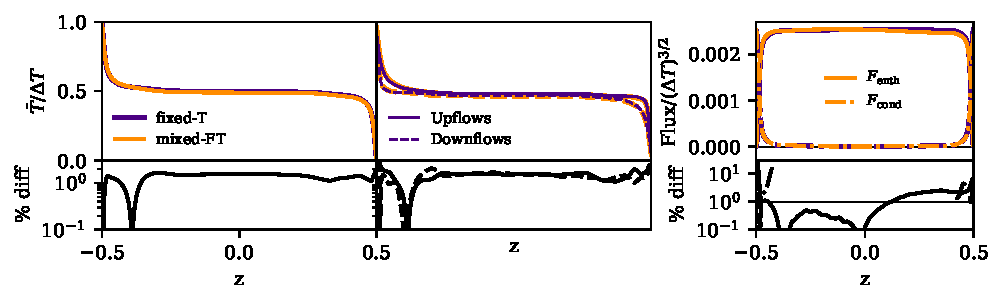
\includegraphics[width=\textwidth]{./figs/rbc_1D_profiles.pdf}
\caption{ 
	(upper left) The horizontally- and time-averaged temperature profile is shown for a mixedFT (green) and fixedT (orange) simulation.
	(upper middle) The horizontally- and time-averaged temperature profile is shown for upflow regions (solid lines) and downflow regions (dashed lines) respectively.
	(upper right) The horizontally- and time-averaged fluxes in the system are shown.
	(bottom panels) The percentage difference between the corresponding quantities in the top panels are displayed, and in most cases measurements agree to within a few percent through the full depth of the domain.
\label{fig:rbc_1D_profiles} }
\end{figure}

In Fig.~\ref{fig:rbc_1D_profiles}, we compare the horizontally averaged, vertical profiles of our fixed-T and mixed-FT cases.
In the upper left panel, we show the mean temperature profiles achieved in the evolved state of both simulations.
Throughout the full depth, these profiles differ by less than 2\%, as shown in the lower left panel.
In the upper middle panel, we show the mean temperature profile in downflow areas compared to the mean temperature profile achieved in upflow areas.
Surprisingly, despite symmetrical boundary conditions in fixed-T simulations and asymmetrical boundary conditions in mixed-FT cases, we find precisely the same asymmetries in upflows/downflows for both sets of boundary conditions.
In general, we find that the boundary layer in upflows is more gradual in hot plumes, and the same is true for downflows and cold plumes.
Once again, these profiles agree to within $< 2\%$.

In the upper right panel of Fig.~\ref{fig:rbc_1D_profiles}, we plot the system fluxes for both cases.
The fluxes show very good agreement just like the temperature profile.
Throughout the bulk of the domain, the convective enthalpy fluxes agree to within a few \% or less (solid line in bottom right panel).
Due to the conductive fluxes approaching zero in the interior, we cannot measure a \% difference for this flux in the bulk, but we find that it is again within a few percent in the boundary layers.

\begin{figure}
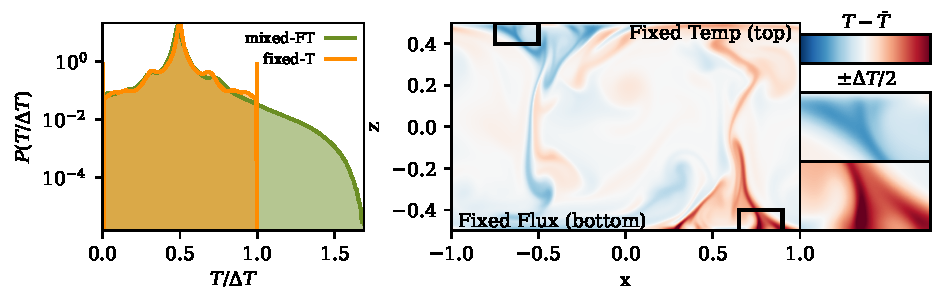
\includegraphics[width=\textwidth]{./figs/rbc_dynamics_asymmetries.pdf}
\caption{ 
	(left panel) PDFs of temperature measurements of a mixedFT (green) and fixedT (orange) case are displayed.
	The right tail of the distribution (near the cold fixed-flux boundary for the mixedFT case) shows that fixed flux boundaries achieve more extreme temperature events than fixed temperature boundaries.
	(middle panel) A snapshot of the temperature anomaly in a mixedFT simulation.
	The black outline boxes around the roots of the plumes are expanded in the bottom right panels.
	Near the top (fixed temperature) boundary, the temperature anomaly at the root of the plume vanishes near the boundary, but this does not happen near the bottom (fixed flux) boundary, allowing for more extreme instantaneous values.
\label{fig:rbc_dynamics_asymmetries} }
\end{figure}

In Fig.~\ref{fig:rbc_dynamics_asymmetries}, we examine the dynamical nature of the asymmetries which mixedFT boundaries introduce into the simulation.
In the left panel, we plot PDFs of the temperature fields in comparable fixedT and mixedFT simulations.
These PDFs agree remarkably well for cold temperatures (near the shared fixed-T boundary) and through the mean, but diverge in the tail of the PDF for hot temperatures (where the boundary conditions differ).
We find that the mixedFT pdf has a much longer tail and is capable of achieving much hotter instantaneous temperature values than a fixedT simulation.
In order to understand how this is possible, we examine a snapshot of the full temperature field.
In the middle panel, we plot the temperature anomaly -- the temperature field with the mean vertical profile subtracted from it.
We have outlined a portion of a cold plume near the upper (fixed-temperature) boundary and a portion of a hot plume near the lower (fixed-flux) boundary, and these regions are magnified in the lower right panels.
The fixed-T upper boundary suppresses temperature anomaly at the upper boundary and regulates the temperature minima which can be achieved.
The fixed-flux lower boundary does no such suppression and allows for extreme temperature values to be achieved in the plume-launching area, thus allowing for the asymmetry in the tails of the temperature PDF.

We note briefly that these asymmetries do not seem to affect mean or volume-averaged quantities in these simulations appreciably (see the agreement between mixedFT and fixedT in Figs.~\ref{fig:rbc_scalar_comparisons}\&\ref{fig:rbc_1D_profiles}).
However, the fact that fixed-flux boundaries produce a wider temperature distribution with more extreme values may be important in some astrophysical studies.
For example, some authors have aimed to quantify the statistical distribution of penetrative plumes from a convective region into a stable region \cite{pratt&all2017}, with implications for the solar dynamo.
These results suggest that the choice of imposed boundary conditions can affect the extreme events that a simulation is capable of achieving.





\section{Rotating \RB Convection}
\label{sec:rotating_results}
We now extend our study of 2D RBC to a more complicated experiment.
Here, we examine rotating RBC with an Ekman number of $10^{-6}$.
We study a fixedT case whose supercriticality is $\sim 3$ with Ra$_{\Delta T} = 2.75\times 10^9$, and a corresponding mixedFT case with $\text{Ra}_{\partial_z T} = 2.1 \times 10^{10}$.
We furthermore employ stress free boundary conditions which allow for the generation of mean flows such as large scale vortices \cite{couston&all2019}.

In the left three panels of Fig.~\ref{fig:rotating_panels}, we once compare the time evolution of the mixedFT and fixedT cases.
The top left panel shows the evolution of Ra$_{\partial_z T}$ and Ra$_{\Delta T}$.
Even in the presence of strong rotation, the fixedT case's fluxes immediately equilibrate, but the mixedFT case takes thousands of freefall times to achieve thermal relaxation.
In the middle left panel, we show the evolution of the Rossby number.
While the evolved states of both simulations exhibit rotationally constrained dynamics with Ro$\sim 0.1$, the initial state of the mixedFT simulation is only weakly rotationally constrained (Ro$\sim 1$).
The degree of rotational constraint felt by the flows decreases slowly toward its final state over thousands of freefall times.
In the bottom left panel, we display the evolution of the Peclet number over time.
Somewhat surprisingly, the peak value of Pe is found not during the convective transient but rather a few hundreds of freefall times later.
After achieving this peak value, the mean Pe monotonically decreases toward its final state.
We suspect that initially large value of Ra$_{\Delta T}$ in the mixedFT case drives high velocity flow associated with a developed large scale vortex (LSV).
As Ra$_{\Delta T}$ and convective driving decrease over time, the driving of the kinetic energy in this LSV eventually reaches an equilibrium value before decreasing, leading to the ``bump'' in the Pe trace.

In the upper right panel of Fig.~\ref{fig:rotating_panels}, we plot the evolution of Nu(t) vs. Ra(t) for our mixedFT case (thick green line) and the evolved value of Nu in the fixedT case (orange star).
We have additionally plotted data from numerical simulations (circles) and experiments (diamonds) as reported in the appendix tables of \cite{cheng&all2015}.
We note that these comparison values are in cylindrical domains with Pr=7, whereas we are in Cartesian geometry with Pr=1, some some differences are expected.
The evolution of Nu vs Ra is very steep compared to the nonrotating RBC cases in Fig.~\ref{fig:rbc_scalar_comparisons}.
Although the simulation details of mixedFT simulations are not, on average, useful, this case of rotating convection is one case where they could be.
The scaling of Nu vs Ra in the rotationally constrained regime is poorly understood [cite, cite], but a single mixedFT simulation can trace through a large portion of this rotationally constrained parameter space.
The evolution of these simulation could therefore perhaps be used to understand how the nature of convection changes as it develops into an increasingly rotationally constrained regime.
However, we once again caution the reader that if they are primarily intersted in the evolved simulation dynamics, then the transient dynamics can be very misleading.
Not only does the mixedFT transient state exhibit more turbulence and heat transport than an evolved state, but the degree of rotational constraint -- and therefore the dominant scale of convection -- also changes appreciably over time.

In the bottom right panels of Fig.~\ref{fig:rotating_panels}, we examine the evolution of dominant flow structures over the course of thermal relaxation.
Shown is the vertically integrated vertical component of the vorticity.
As shown in the left panel, a dominant LSV which is aligned with the global rotation forms at early times.
Over thousands of freefall times, this LSV evolves into a long-lived vortex pair, displayed in the middle panel.
Finally, in the evolved state, this vortex pair solution begins to oscillate with domain-wide jets, such as those displayed in the right panel.
We find that the the fixedT solution shows this oscillatory behavior between vortex pairs and jets immediately and throughout the full 5000 frefall timescales of evolution that we simulated.

Importantly, the convective transient of the mixedFT simulation studied here requires significantly higher spectral resolution to resolve than the evolved state.
The fixedT simulation shown in this section was computed stably at $128^3$.
On the other hand, the convective transient of the mixedFT simulation was computed at $512\times384^2$.
In order to reduce the computational cost of this simulation, we reduced the vertical resolution twice as the simulation became more rotationally constrained.
One hundred freefall times after transient, we reduced the resolution to $256\times384^2$.
About $3.3 \times 10^3$ freefall times into the simulation, we further reduced the vertical resolution to $128\times384^2$.
At each of these times, we found that the simulation solution could not be reproduced with fidelity upon lowering the horizontal resolution.
This suggests that small scale turbulent velocity structure injected by the vigorous transient is long lived throughout the thermal evolution of the simulation.

We also note that the difference in computational cost required to reach the equilibrated solution is staggering.
The number of iteration per cpu-hour was 4.25 at $512\times384^2$, 10.6 at $256\times384^2$, and 38 at $128\times384^2$.
The first resolution was run for $1.59 \times 10^5$ iterations, the second for $2.22 \times 10^6$ iterations, and the third for $3.30 \times 10^6$ iterations.

On the other hand, the fixedT simulation got 56.4 iterations per cpu-hour, and ran for $1.46 \times 10^6$ iterations, for $\sim 2.6 \times 10^4$ cpu-hours.





\begin{figure}
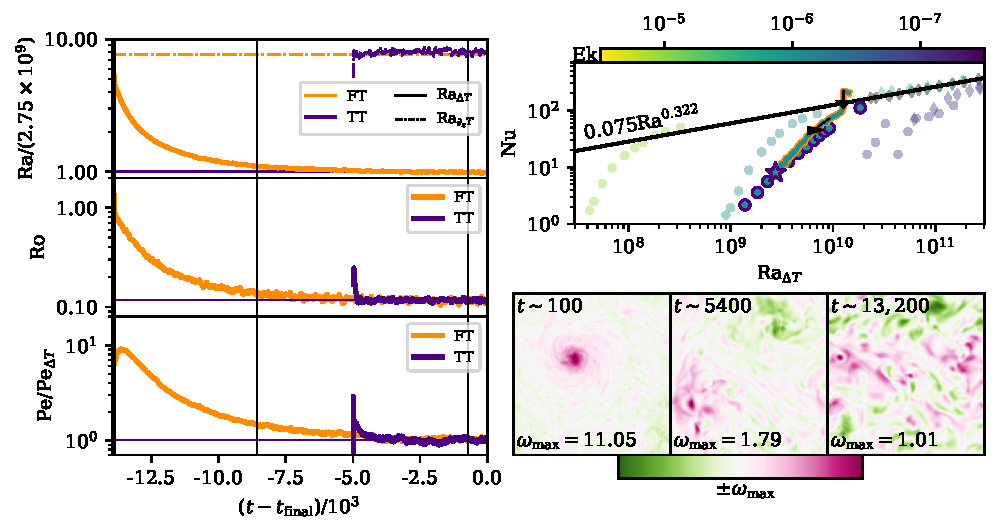
\includegraphics[width=\textwidth]{./figs/rotating_panels.pdf}
\caption{ 
	(left panel) PDFs of temperature measurements of a mixedFT (green) and fixedT (orange) case are displayed.
	The right tail of the distribution (near the cold fixed-flux boundary for the mixedFT case) shows that fixed flux boundaries achieve more extreme temperature events than fixed temperature boundaries.
	(middle panel) A snapshot of the temperature anomaly in a mixedFT simulation.
	The black outline boxes around the roots of the plumes are expanded in the bottom right panels.
	Near the top (fixed temperature) boundary, the temperature anomaly at the root of the plume vanishes near the boundary, but this does not happen near the bottom (fixed flux) boundary, allowing for more extreme instantaneous values.
\label{fig:rotating_panels} }
\end{figure}


%%%%%%%%%%%%
%%%%%%%%%%%
% CONCLUSION
%%%%%%%%%%%
%%%%%%%%%%%%

\section{Discussion \& Conclusions}
\label{sec:discussion}

Here we basically say everything we said again, but in short form, and then we perhaps talk about the implications for astrophysics.
Doesn't hurt to repeat all of the imprtant points we made all over again.


\begin{acknowledgments}
We'd like to thank Daniel Lecoanet, who first pointed out to us the importance of examining Ra$_{\Delta T}$ in mixedFT simulations. 
EHA acknowledges that this work was supported by NASA Headquarters under the NASA Earth and Space Science Fellowship Program -- Grant 80NSSC18K1199.
This work was additionally supported by NASA LWS grant NNX16AC92G and by the National Science Foundation under grant No.~1616538. 
Computations were conducted with support by the NASA High End Computing (HEC) Program through the NASA  Advanced Supercomputing (NAS) Division at Ames Research Center on Pleiades with allocation GID s1647.
\end{acknowledgments}


\bibliography{biblio.bib}

\appendix
\section{Table of Simulations}
\label{app:table}


\begin{table}[ht]
\caption{
	Input and output values from the simulations in this work are shown.
	The ``Nu comp'' values are comparison Nusselt number values reported in \cite{zhu&all2018}.
	Values of Nu and Re are the sample mean; the standard deviation of the sample mean is shown for Nu measurements, and is smaller than the number of significant figures reported for Re measurements.
}
\setlength{\tabcolsep}{12pt}
\label{table:speed}
\begin{center}
\begin{tabularx}{\textwidth}{c c c c c c c c c}
\hline																	
BCs	&	Ra	&	Pr	&	Ek	&	nz$\times$nx$\times$ny	&	cpu-hours &	Nu	&	Nu comp	&	Re \\
%\hline \hline \multicolumn{6}{c}{\vspace{-0.2cm}}\\
%\multicolumn{6}{c}{\vspace{0.1cm}2D Runs} \\
\hline
fixedT	&	$1.00 \times 10^8$	&	1	&	$\infty$	&	512x1024	&	$5.57 \times 10^3$	&	$25.4 \pm 0.1$	&	26.1	&	$3.18 \times 10^3$ \\
mixedFT	&	$2.61 \times 10^9$	&	1	&	$\infty$	&	1024x2048	&	$1.21 \times 10^5$	&	$25.3 \pm 0.2$	&	26.1	&	$3.31 \times 10^3$ \\
fixedT	&	$2.15 \times 10^8$	&	1	&	$\infty$	&	512x1024	&	$5.73 \times 10^3$	&	$31.3 \pm 0.2$	&	31.2	&	$5.17 \times 10^3$ \\
fixedT	&	$4.64 \times 10^8$	&	1	&	$\infty$	&	1024x2048	&	$4.66 \times 10^4$	&	$38.4 \pm 0.3$	&	38.9	&	$8.60 \times 10^3$ \\
fixedT	&	$1.00 \times 10^9$	&	1	&	$\infty$	&	1024x2048	&	$5.58 \times 10^4$	&	$48.0 \pm 0.4$	&	48.3	&	$1.33 \times 10^4$ \\
fixedT	&	$2.15 \times 10^9$	&	1	&	$\infty$	&	1024x2048	&	$6.38 \times 10^4$	&	$60.4 \pm 0.5$	&	61.1	&	$1.99 \times 10^4$ \\
\hline																	
\hline																	
fixedT	&	$2.75 \times 10^9$		&	1	&	$10^{-6}$	&	128$^3$				&	?					&	$8.04 \pm 0.01$	&	---		&	$1.71 \times 10^3$ \\
mixedFT	&	$2.1 \times 10^{10}$	&	1	&	$10^{-6}$	&	nz$\times$384$^2$	&	?					&	$7.86 \pm 0.01$	&	---		&	$1.76 \times 10^3$ \\
\hline																	
\end{tabularx}
\end{center}
\end{table}



\end{document}
